\section{Methods}
\begin{center}
    \begin{figure}
    \makebox[\textwidth]{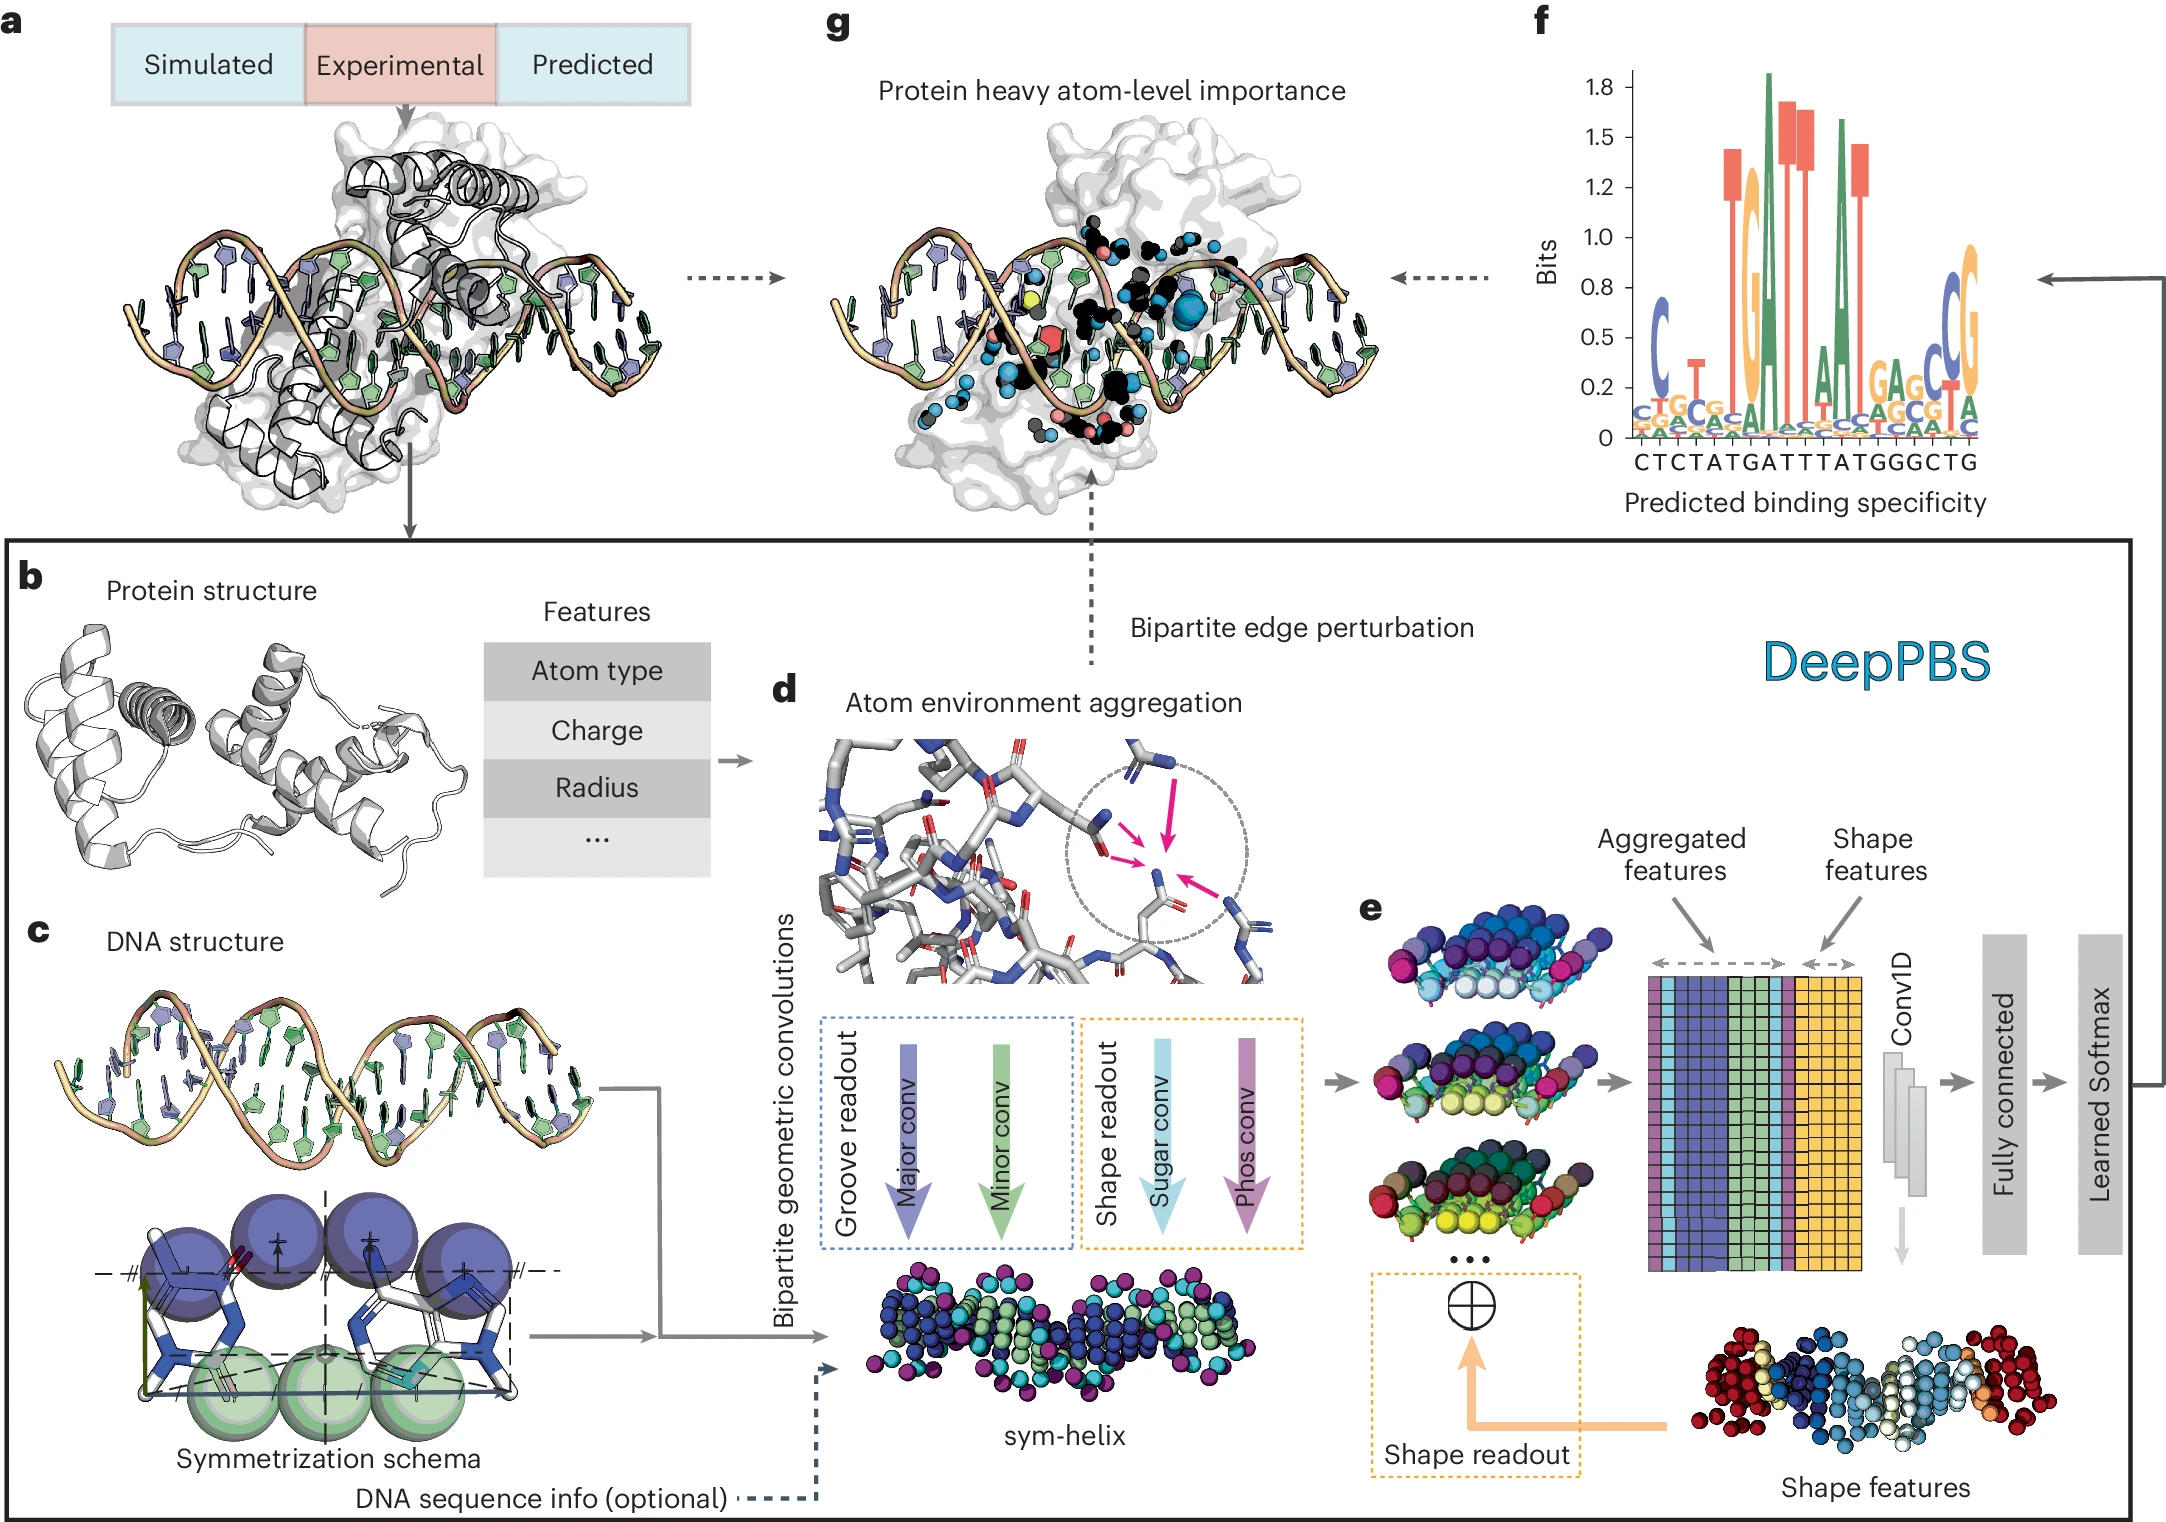
\includegraphics[width=0.8\paperwidth]{./pdna_figs/fig1.png}}
 % archetecture.png: 1149x508 px, 72dpi, 40.53x17.92 cm, bb=0 0 1149 508
        \caption[Computational cost of training RVAgene]{\textbf{Training RVAgene is reasonably scalable on CPU and even more so using hardware acceleration through GPU.} ({\bf A}) Time cost of training RVAgene for 100 epochs for datasets with varying number of genes and time points on CPU and GPU. ({\bf B}) Maximum memory utilized during training of the model on CPU an GPU for the cases in (A), inset plot: comparison of max memory used compared to DPGP for varying number of genes.}
  \label{fig:pdna7}
\end{figure}
\end{center}


\begin{center}
    \begin{figure}
    \makebox[\textwidth]{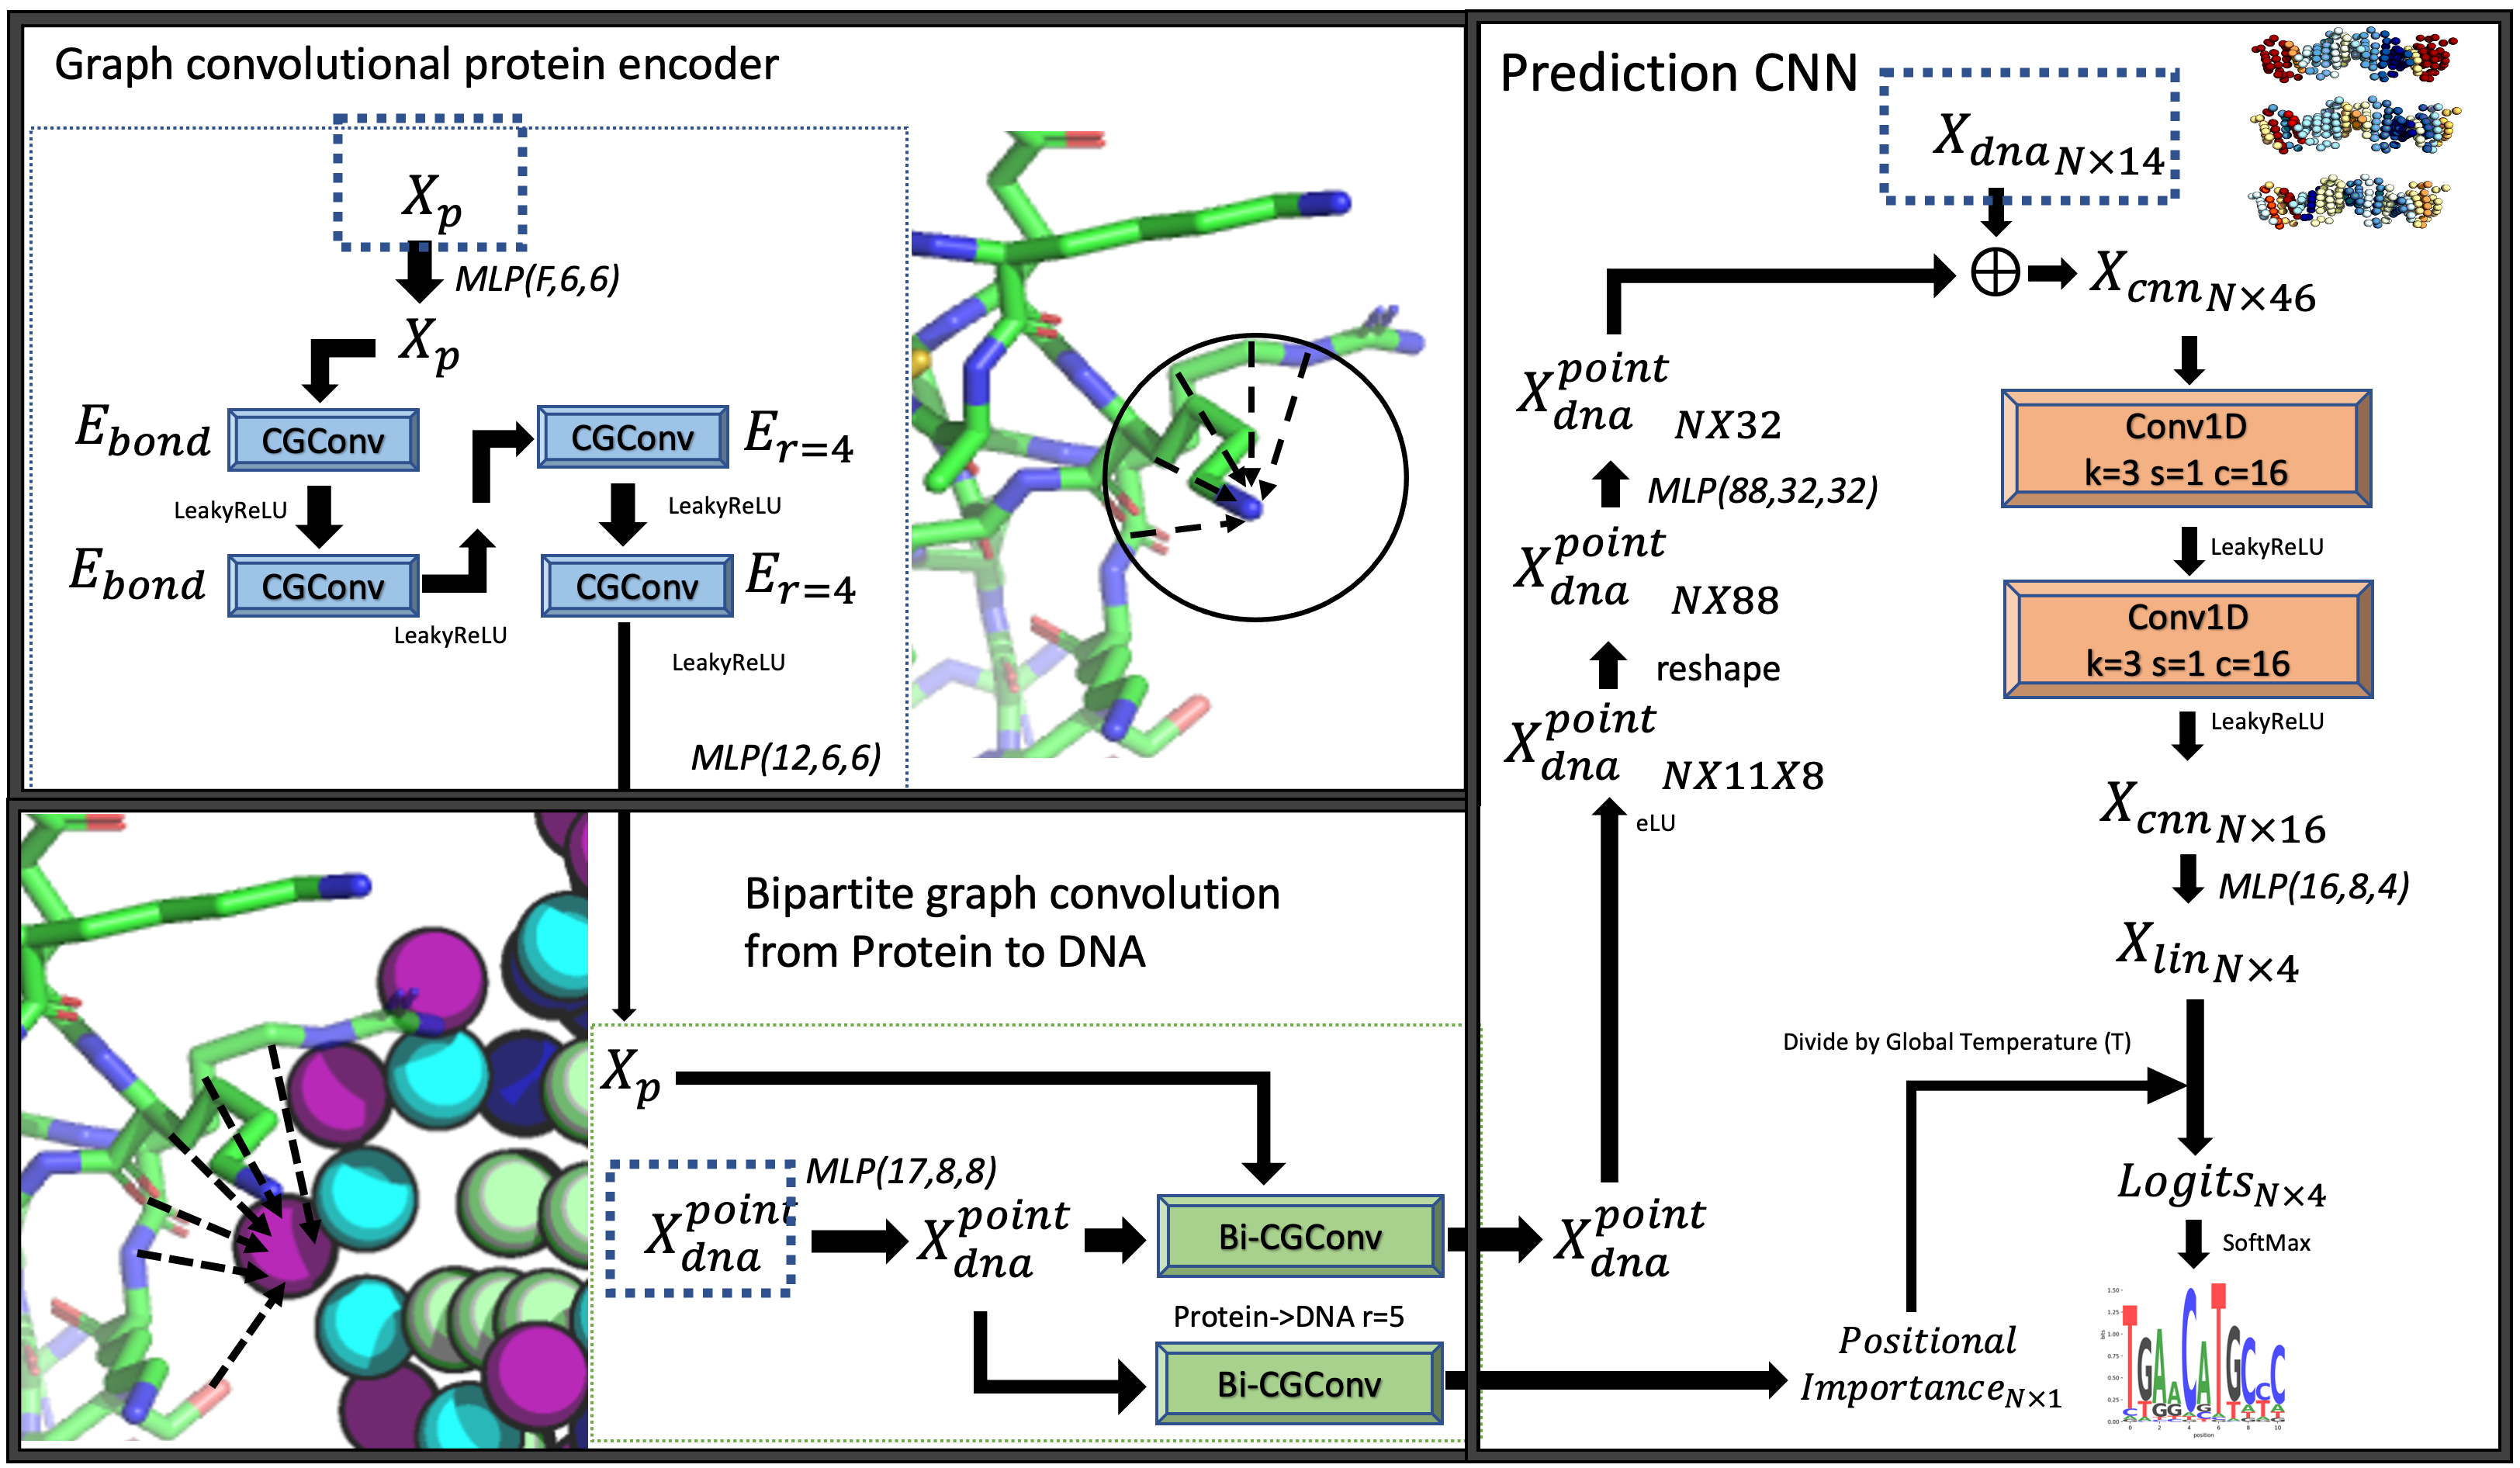
\includegraphics[width=0.8\paperwidth]{./pdna_figs/fig2.png}}
 % archetecture.png: 1149x508 px, 72dpi, 40.53x17.92 cm, bb=0 0 1149 508
        \caption[Computational cost of training RVAgene]{\textbf{Training RVAgene is reasonably scalable on CPU and even more so using hardware acceleration through GPU.} ({\bf A}) Time cost of training RVAgene for 100 epochs for datasets with varying number of genes and time points on CPU and GPU. ({\bf B}) Maximum memory utilized during training of the model on CPU an GPU for the cases in (A), inset plot: comparison of max memory used compared to DPGP for varying number of genes.}
  \label{fig:pdna7}
\end{figure}
\end{center}
